\chapter{TEORIA DAS PROBABILIDADES}
\section{Introdução}

A Teoria dos Conjuntos é uma das áreas fundamentais da Matemática,
responsável pelo estudo das propriedades e relações entre coleções de objetos,
denominadas \textit{conjuntos}. Sua origem está associada principalmente aos
trabalhos do matemático alemão \textbf{Georg Ferdinand Ludwig Philipp Cantor}
(1845--1918), considerado o fundador da teoria moderna dos conjuntos. \vskip0.3cm

Cantor introduziu a ideia de que um conjunto pode ser tratado como uma noção
primitiva, isto é, um conceito básico que não necessita de definição formal
imediata. Por esse motivo, a teoria inicial ficou conhecida como
\textit{teoria ingênua dos conjuntos}. No entanto, essa abordagem revelou
diversas antinomias (ou paradoxos), que surgiram devido à ausência de uma base
axiomática rigorosa para definir conjuntos arbitrários.
\vskip0.3cm

Esses paradoxos conduziram a Matemática, ao longo do século XX, a um processo
de \textbf{axiomatização}, influenciando profundamente os fundamentos da lógica
e da própria Matemática.

\begin{figure}
    \centering
    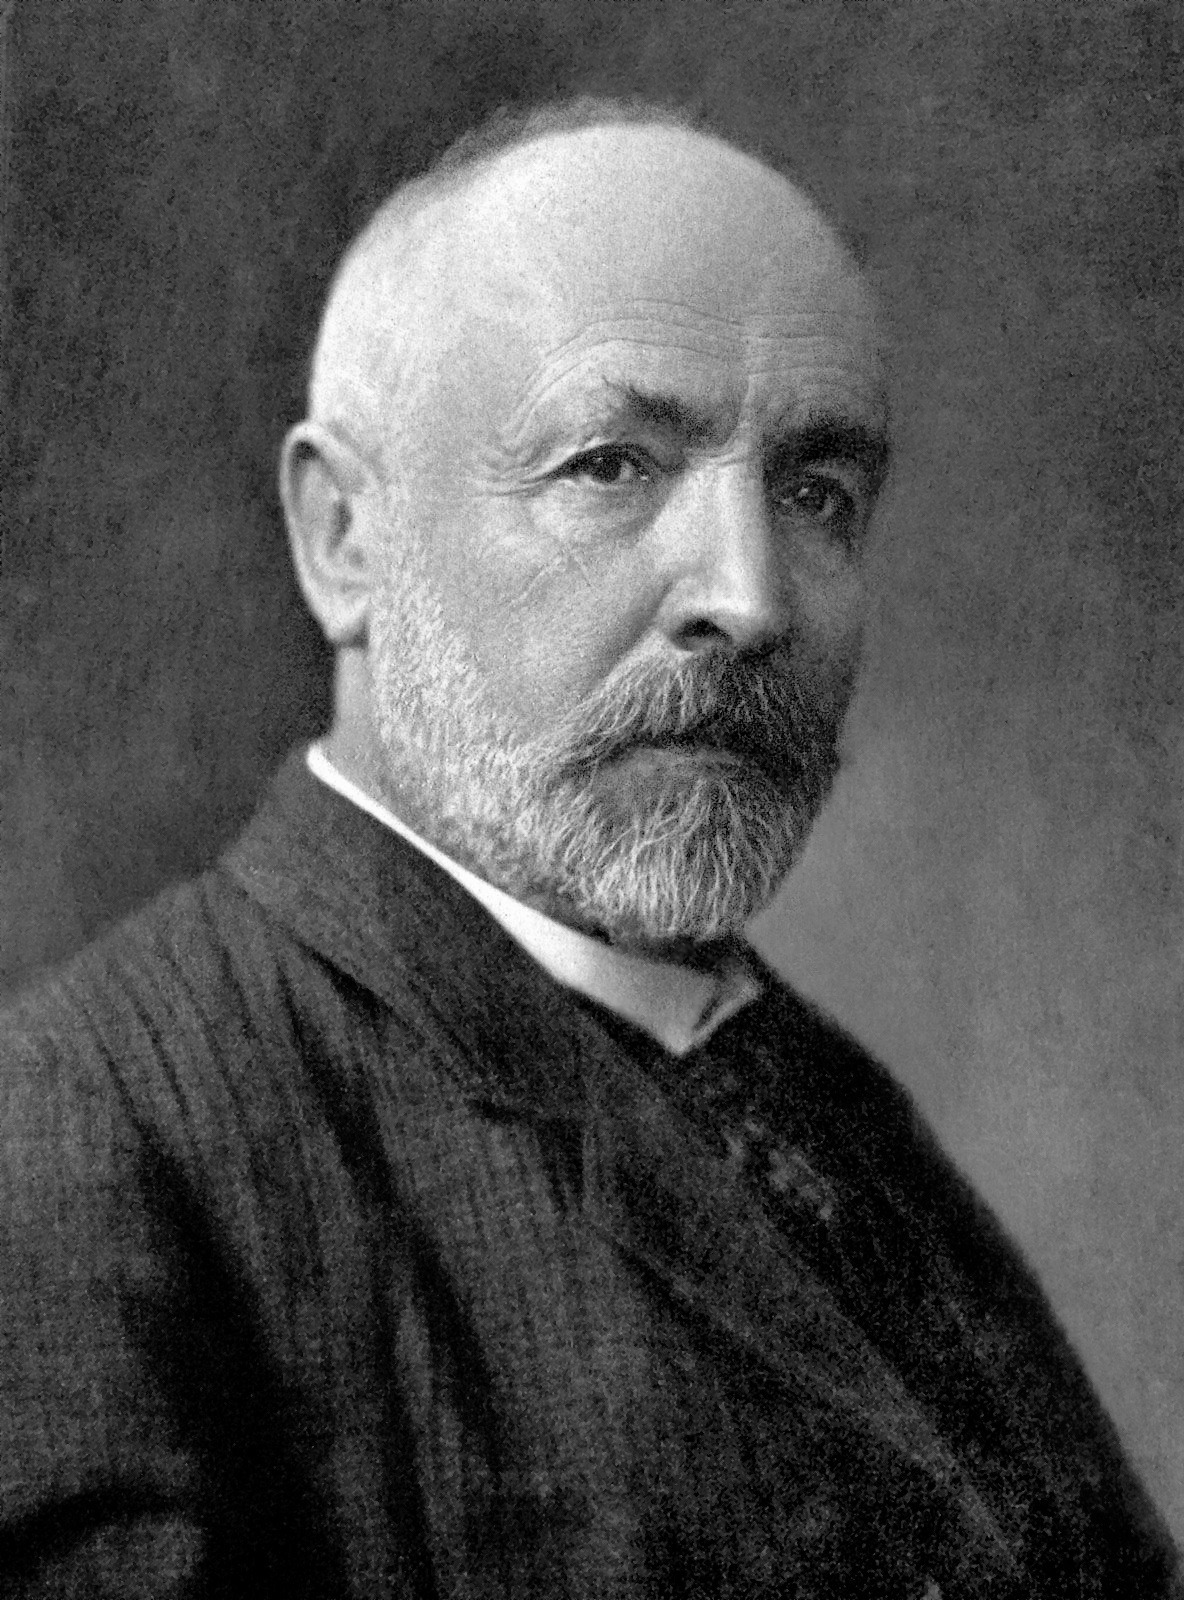
\includegraphics[scale=0.066]{figures/Cantor1.jpeg}
    \caption{Georg Ferdinand
Ludwig Philipp Cantor(1845-1918)}
    \label{fig:my_label}
\end{figure}

\newpage
A teoria teve início formal com a publicação, em 1874, de um artigo no qual
Cantor investigava a comparação entre coleções infinitas. Uma de suas grandes
contribuições foi demonstrar que conjuntos infinitos podem possuir diferentes
``tamanhos'', conceito hoje conhecido como \textit{cardinalidade}.
\vskip0.3cm

Desde 1638, com \textbf{Galileu Galilei}, já se sabia que é possível estabelecer
uma correspondência biunívoca entre os números inteiros e seus quadrados,
contrariando a concepção euclidiana de que ``o todo é sempre maior que qualquer
uma de suas partes''.
\vskip0.3cm

Cantor utilizou esse princípio para desenvolver o método da diagonalização,
com o qual provou, por contradição, que o conjunto dos números reais não admite
uma correspondência biunívoca com o conjunto dos números inteiros. Esse resultado
contribuiu para o desenvolvimento do conceito de contínuo, posteriormente
formalizado por \textbf{Richard Dedekind}.
\vskip0.3cm

Em 1892, Cantor demonstrou que o conjunto dos números racionais
$\mathbb{Q}$ é enumerável, enquanto o conjunto dos números reais
$\mathbb{R}$ é não enumerável, portanto de cardinalidade maior.
Mais tarde, em 1897, surgiram paradoxos associados à teoria, motivando o avanço
dos sistemas axiomáticos.
\vskip0.3cm

Apesar das críticas enfrentadas em vida, suas ideias foram plenamente assimiladas
e tornaram-se essenciais em diversos ramos da Matemática moderna.

%\newpage
\section{Conjuntos}

O conceito de conjunto é fundamental não apenas para a Probabilidade e a Estatística,
mas para toda a Matemática. \vskip0.3cm

\textit{Qualquer coleção bem definida de objetos é chamada de conjunto}.
Os objetos que compõem um conjunto são chamados de \textit{elementos} ou
\textit{membros}.
\vskip0.3cm

Em geral, denotamos conjuntos por letras maiúsculas $(A,B,C,\dots)$
e seus elementos por letras minúsculas $(a,b,c,\dots)$.


\newpage
\section{Subconjuntos}

Se todo elemento de um conjunto $A$ também pertence a um conjunto $B$,
dizemos que $A$ é subconjunto de $B$, e escrevemos:

\[
A \subseteq B
\]

ou equivalentemente:

\[
B \supseteq A.
\]

Se um elemento $a$ pertence ao conjunto $C$, escrevemos:

\[
a \in C.
\]

Caso contrário:

\[
a \notin C.
\]

Um conjunto é considerado bem definido quando existe uma regra clara que permita
decidir se um determinado objeto pertence ou não a ele.
\vskip0.3cm

Existem diferentes formas de descrever um conjunto:

\begin{enumerate}
    \item Listando explicitamente seus elementos:
    \[
    A = \{1,2,3,4\}.
    \]

    \item Descrevendo-o verbalmente:
    ``o conjunto de todos os números reais entre 0 e 1''.

    \item Utilizando notação por propriedade:
    \[
    A = \{x \mid 0 \leq x \leq 1\}.
    \]
\end{enumerate}

\newpage
\section{Experimentos Aleatórios}

Um \textbf{experimento aleatório} é aquele que, mesmo repetido sob condições
idênticas, pode produzir resultados diferentes, sem que seja possível prever com
certeza o resultado individual.
\vskip0.3cm

\begin{itemize}
\item Exemplo 1: Lançar uma moeda três vezes. \\
\item Exemplo 2: Lançar dois dados simultaneamente.
\end{itemize}

\vskip0.3cm

\subsection{Características dos Experimentos Aleatórios}

\begin{itemize}
    \item Podem ser repetidos indefinidamente sob as mesmas condições;
    \item Não se pode prever um resultado específico, mas é possível listar todos
    os resultados possíveis;
    \item Quando repetidos muitas vezes, apresentam regularidade estatística nas frequências observadas.
\end{itemize}



\section{Fenômenos Aleatórios}

Fenômenos aleatórios diferem dos experimentos aleatórios porque, em geral,
não podem ser controlados ou reproduzidos livremente: o pesquisador atua como
observador. \vskip0.3cm

Fenômenos estudados pela Estatística possuem \textit{regularidade estatística},
ou seja, podem ser observados repetidamente ao longo do tempo. \vskip0.3cm


\begin{itemize}
\item Exemplo 1: Número mensal de casos de meningite em Belém. \\
\item Exemplo 2: Quantidade mensal de chuva em uma região.
\end{itemize}

\newpage
\section{Espaço Amostral}

O \textbf{espaço amostral}, denotado por $S$ ou $\Omega$, é o conjunto de todos
os resultados possíveis de um experimento aleatório.
\vskip0.3cm

Por exemplo, ao lançar dois dados, o espaço amostral contém $36$ pares ordenados:

\[
\Omega = \{(i,j)\mid i=1,\dots,6,\ j=1,\dots,6\}.
\]



\subsection{Espaço Amostral Discreto}

Quando os resultados possíveis são finitos ou enumeráveis, dizemos que o espaço
amostral é \textbf{discreto}:

\[
\Omega = \{w_1,w_2,w_3,\dots\}.
\]


\subsection{Espaço Amostral Contínuo}

Quando os resultados possíveis são não enumeráveis, geralmente associados a
mensurações (tempo, peso, altura), o espaço amostral é \textbf{contínuo}.


\section{Eventos}

Um \textbf{evento} é qualquer subconjunto do espaço amostral $\Omega$. \vskip0.3cm

Os eventos podem ser simples ou compostos e são representados por letras maiúsculas.

\subsection{Operações com Eventos}

Sejam $A$ e $B$ eventos em $\Omega$:

\begin{enumerate}
    \item União:
    \[
    A \cup B
    \]
    ocorre se $A$ ou $B$ ocorrer (ou ambos).

    \item Interseção:
    \[
    A \cap B
    \]
    ocorre se $A$ e $B$ ocorrerem simultaneamente.

    \item Complementar:
    \[
    A^c
    \]
    ocorre se $A$ não ocorrer.

    \item Diferença:
    \[
    A - B
    \]
    representa os resultados que estão em $A$, mas não em $B$.

    \item Eventos mutuamente exclusivos:
    \[
    A \cap B = \varnothing.
    \]
\end{enumerate}

\subsection{Propriedades das Operações}

\begin{enumerate}
    \item Comutatividade:
    \[
    A \cup B = B \cup A,
    \qquad
    A \cap B = B \cap A.
    \]

    \item Associatividade:
    \[
    A \cup (B \cup C) = (A \cup B)\cup C,
    \]
    \[
    A \cap (B \cap C) = (A \cap B)\cap C.
    \]

    \item Distributividade:
    \[
    A \cup (B \cap C) = (A \cup B)\cap (A \cup C),
    \]
    \[
    A \cap (B \cup C) = (A \cap B)\cup (A \cap C).
    \]

    \item Leis de De Morgan:
    \[
    (A \cup B)^c = A^c \cap B^c,
    \qquad
    (A \cap B)^c = A^c \cup B^c.
    \]

    \item Propriedades gerais:
    \[
    A \cup \varnothing = A,
    \qquad
    A \cap \varnothing = \varnothing,
    \]
    \[
    (A^c)^c = A,
    \qquad
    A \cup A^c = \Omega.
    \]
\end{enumerate}
%----------------------------------------------------------------------------------%


\newpage
%----------------------------------------------------------------------------------%
\section{Definições de Probabilidade}

Historicamente, a probabilidade foi objeto de ampla discussão, tendo sido definida de maneiras distintas ao longo do tempo. Inicialmente, surgiu a definição segundo a qual a probabilidade de um evento é o limite da frequência relativa de sua ocorrência quando o número de repetições do experimento tende ao infinito. Essa concepção, denominada \textbf{frequentista}, apresenta, entretanto, importantes limitações, especialmente quando não é possível repetir o experimento um grande número de vezes.\vskip0.3cm
 
Uma segunda definição, conhecida como \textbf{clássica}, concebe a probabilidade como o quociente entre o número de casos favoráveis a um evento e o número total de casos possíveis, desde que todos sejam igualmente prováveis. Atualmente, essa definição é considerada uma regra prática útil apenas em situações específicas.\vskip0.3cm

Na segunda metade do século XIX, a Teoria das Probabilidades atingiu um de seus pontos mais altos com os trabalhos da escola russa fundada por \textbf{Pafnuty Lvovich Chebyshev} (1821--1894).\vskip0.3cm
 
Modernamente, adota-se a definição \textbf{axiomática} da probabilidade, proposta em 1933 pelo matemático russo \textbf{Andrei Nikolaevich Kolmogorov}, segundo a qual a probabilidade deve obedecer a três axiomas fundamentais.


 

\subsection{Definição Frequentista de Probabilidade}

Na prática, nem sempre é possível determinar exatamente a probabilidade de um evento. Nesses casos, utiliza-se um método de aproximação baseado na repetição do experimento aleatório. Esse procedimento permite estimar a probabilidade de um evento $A$ a partir de dados observados. A probabilidade avaliada dessa forma é denominada \textbf{probabilidade empírica}.\vskip0.3cm

Seja $\epsilon$ um experimento aleatório e $A$ um evento do espaço amostral $S$ associado a esse experimento. Suponha que $\epsilon$ seja repetido $n$ vezes e que $m$ seja o número de vezes em que $A$ ocorre. A frequência relativa do evento $A$, denotada por $f_{r_A}$, é definida como:

\begin{equation}
     f_{r_A}= \frac{m}{n}.
\end{equation}

\subsubsection{Propriedades da Frequência Relativa} 

Seja $\epsilon$ um experimento aleatório e $A$ e $B$ dois eventos do espaço amostral $S$. Sejam $f_{r_A}$ e $f_{r_B}$ as frequências relativas de $A$ e $B$, respectivamente. Então:

\begin{enumerate}
    \item $0 \leqslant f_{r_A} \leqslant 1$, isto é, a frequência relativa de um evento varia entre $0$ e $1$.
    
    \item $f_{r_A}=1$ se, e somente se, $A$ ocorre em todas as $n$ repetições de $\epsilon$.
    
    \item $f_{r_A}=0$ se, e somente se, $A$ não ocorre em nenhuma das $n$ repetições de $\epsilon$.
    
    \item Se $A$ e $B$ forem mutuamente excludentes, então:
    \[
    f_{r_{A \cup B}} = f_{r_A} + f_{r_B}.
    \]
\end{enumerate}


\subsection{Definição Clássica de Probabilidade}
 

Seja $E$ um experimento aleatório e $S$ um espaço amostral formado por $n$ resultados igualmente prováveis. Seja $A \subseteq S$ um evento com $m$ elementos. A probabilidade de $A$, denotada por $P(A)$, é definida como:

\begin{equation}
     P(A)= \frac{m}{n}.
\end{equation}
  
Isto é, a probabilidade do evento $A$ é o quociente entre o número de casos favoráveis e o número de casos possíveis.\vskip0.3cm

\textbf{Exemplo:} Calcular a probabilidade de, no lançamento de um dado equilibrado, obter-se:

\begin{enumerate}
    \item Um resultado igual a $4$.
    \item Um resultado ímpar.
\end{enumerate}

\[
P(A)= \frac{1}{6} \approx 16,67\%.
\]

\[
P(B)= \frac{3}{6} = 50\%.
\]

A definição clássica apresenta limitações, pois a noção de ``igualmente provável'' já pressupõe o conceito de probabilidade, tornando a definição parcialmente circular. Além disso, ela não se aplica quando o espaço amostral é infinito ou quando os resultados não são equiprováveis.


\subsection{Definição Axiomática de Probabilidade}
\subsubsection{O Que é Axiomática?}

Em determinado estágio da evolução de uma teoria matemática, torna-se necessário ordenar, sistematizar e relacionar todos os conhecimentos nela reconhecidos, isto é, proceder à sua \textbf{axiomatização}.\vskip0.3cm
 
Axiomatizar consiste em:

\begin{enumerate}
\item Escolher afirmações fundamentais sobre os objetos matemáticos em estudo;
\item A partir delas, deduzir todas as demais proposições da teoria por raciocínio lógico.
\end{enumerate} 

Essas afirmações fundamentais são denominadas \textbf{axiomas}, e o conjunto delas constitui uma \textbf{axiomática}.\vskip0.3cm
 

Os axiomas devem ser:

\begin{enumerate}
    \item \textbf{Logicamente independentes}, isto é, nenhum deles deve ser deduzido dos demais;
    \item \textbf{Compatíveis}, ou seja, não podem conduzir a contradições.
\end{enumerate}
 
As proposições deduzidas a partir dos axiomas são chamadas \textbf{teoremas}.\vskip0.3cm

\newpage
Em 1933, \textbf{Andrei Nikolaevich Kolmogorov} estabeleceu a formulação axiomática moderna da probabilidade em sua obra \textbf{Foundations of the Theory of Probability}. Sua construção foi baseada nas propriedades das frequências relativas e nas operações da teoria dos conjuntos.

\begin{figure}
    \centering
    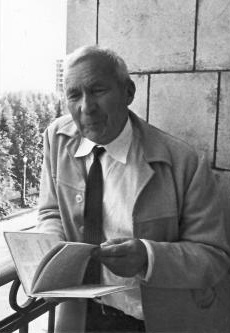
\includegraphics[scale=0.65]{figures/Kolmogorov.jpeg}
    \caption{Andrei Nikolaevich Kolmogorov (1903-1987)}
    \label{fig:my_label10}
\end{figure}

Kolmogorov nasceu em 25 ade abril de 1903 em Tambov, na cidade de Moscou. Foi um matemtático Russo, participou das maiores descobertas científicas do século XX, nas áreas de Probabilidade e Estatística, e em Teoria da Informação.\vskip0.3cm

Considerado um dos grandes cientista em sua época, Kolmogorov foi agraciado por diversas honrarias ao longo de sua carreira:

\begin{itemize}
\item Prêmio Lenin em 1941;
\item Prêmio Balzan em 1962;
\item Medalha Helmholtz em 195;
\item Prêmio Wolf de Matemática em 1980;
\item Medalha Lobachevsky em 1986;
\end{itemize}


\newpage
\subsubsection{Axiomas de Probabilidade}

Seja $S$ um espaço amostral. A cada evento $A \subseteq S$ associa-se um número real $P(A)$, denominado probabilidade de $A$, que satisfaz:

\begin{enumerate}
    \item \textbf{Não negatividade:} $P(A)\geq 0$.
    
    \item \textbf{Normalização:} $P(S)=1$.
    
    \item \textbf{Aditividade:} Se $A$ e $B$ são eventos mutuamente excludentes, então:
    \[
    P(A\cup B)=P(A)+P(B).
    \]
\end{enumerate}

\subsubsection{Consequências dos Axiomas}

Como consequências diretas desses axiomas, obtêm-se:

\begin{enumerate}
\item $P(\varnothing)=0$.
\item $P(\bar{A})=1-P(A)$.
\item $P(A\cup B)=P(A)+P(B)-P(A\cap B)$.
\item Se $A\subseteq B$, então $P(A)\leq P(B)$.
\end{enumerate}

%------------------------------------------------------------------------------------%
\section{Probabilidade Condicional}

Sejam $A$ e $B$ dois eventos associados a um experimento aleatório $\varepsilon$.
Denotaremos por $P(B\mid A)$ a probabilidade condicional do evento $B$,
isto é, a probabilidade de que $B$ ocorra dado que $A$ já ocorreu.\vskip0.3cm

Sempre que calculamos $P(B\mid A)$, estamos essencialmente avaliando a probabilidade de $B$
em relação a um \textbf{espaço amostral reduzido}, isto é, restrito ao evento $A$,
em vez de considerarmos o espaço amostral original $S$.\vskip0.3cm

Quando calculamos $P(B)$, perguntamos quão provável é estarmos em $B$ sabendo que devemos estar em $S$.
Já ao calcular $P(B\mid A)$, perguntamos quão provável é estarmos em $B$ sabendo que devemos estar em $A$.
Assim, o espaço amostral se reduz de $S$ para $A$.\vskip0.3cm

A probabilidade condicional é definida por:

\begin{equation}
    P(B\mid A)=\frac{P(A\cap B)}{P(A)}, \quad \text{desde que } P(A)>0.
\end{equation}

De forma análoga:

\begin{equation}
    P(A\mid B)=\frac{P(A\cap B)}{P(B)}, \quad \text{desde que } P(B)>0.
\end{equation}

É simples verificar as seguintes propriedades de $P(B\mid A)$, para $A$ fixado:

\begin{enumerate}
    \item $0\leq P(B\mid A)\leq 1$;
    \item $P(S\mid A)=1$;
    \item $P(B_{1}\cup B_{2}\mid A)=P(B_{1}\mid A)+P(B_{2}\mid A)$,
    se $B_{1}$ e $B_{2}$ forem mutuamente excludentes;
    \item Mais geralmente,
    \[
    P\left(\bigcup_{i=1}^{n}B_i \,\Big|\, A\right)=\sum_{i=1}^{n}P(B_i\mid A),
    \]
    se os eventos $B_i$ forem dois a dois mutuamente excludentes.
\end{enumerate}


\textbf{Exemplo 1:} Dois dados equilibrados são lançados e o resultado é registrado como $(x_{1},x_{2})$,
onde $x_i$ representa o resultado do $i$-ésimo dado. Assim, o espaço amostral possui $36$ resultados igualmente prováveis:

\[
\Omega=
\left\{
(x_1,x_2):x_1,x_2\in\{1,2,3,4,5,6\}
\right\}.
\]

Considere os eventos:

\[
A=\{(x_1,x_2):x_1+x_2=10\},
\qquad
B=\{(x_1,x_2):x_1>x_2\}.
\]

Calcular:

\begin{enumerate}
    \item $P(B\mid A)$;
    \item $P(A\mid B)$.
\end{enumerate}

O evento $A$ ocorre nos casos:

\[
(4,6),(5,5),(6,4),
\]

portanto:

\[
P(A)=\frac{3}{36}.
\]

O evento $A\cap B$ ocorre apenas em:

\[
(6,4),
\]

logo:

\[
P(A\cap B)=\frac{1}{36}.
\]

Assim,

\[
P(B\mid A)=\frac{P(A\cap B)}{P(A)}
=\frac{\frac{1}{36}}{\frac{3}{36}}=\frac{1}{3}.
\]

Além disso,

\[
P(B)=\frac{15}{36},
\]

portanto,

\[
P(A\mid B)=\frac{\frac{1}{36}}{\frac{15}{36}}=\frac{1}{15}.
\]

\textbf{Exemplo 2:} Uma caixa contém duas moedas: uma honesta e outra com duas faces ``cara''.
Uma moeda é escolhida aleatoriamente, lançada e o resultado observado é cara.
Qual a probabilidade de que a moeda escolhida seja a moeda de duas caras?\vskip0.3cm

Considere os eventos:

\[
A=\{\text{a moeda escolhida é a de duas caras}\},
\qquad
B=\{\text{o resultado observado é cara}\}.
\]

Temos:

\[
P(A)=\frac{1}{2},\qquad
P(B\mid A)=1,\qquad
P(B\mid A^c)=\frac{1}{2}.
\]

Logo,

\[
P(B)=P(B\mid A)P(A)+P(B\mid A^c)P(A^c)
=1\cdot\frac{1}{2}+\frac{1}{2}\cdot\frac{1}{2}
=\frac{3}{4}.
\]

Assim,

\[
P(A\mid B)=\frac{P(B\mid A)P(A)}{P(B)}
=\frac{1\cdot\frac{1}{2}}{\frac{3}{4}}
=\frac{2}{3}.
\]

\subsection{Teorema da Multiplicação}

Da definição de probabilidade condicional, obtemos:

\[
P(A\cap B)=P(B\mid A)P(A),
\]

ou equivalentemente:

\[
P(A\cap B)=P(A\mid B)P(B).
\]

Esse resultado é conhecido como o \textbf{Teorema da Multiplicação}.\vskip0.3cm

Ele pode ser generalizado para $n$ eventos:

\begin{equation}
P(A_1\cap A_2\cap\cdots\cap A_n)=
P(A_1)\,P(A_2\mid A_1)\cdots P(A_n\mid A_1,\dots,A_{n-1}).
\end{equation}

\subsection{Partição do Espaço Amostral e Probabilidade Total}

Dizemos que os eventos $B_1,B_2,\dots,B_k$ formam uma \textbf{partição} do espaço amostral $S$ se:

\begin{enumerate}
    \item $B_i\cap B_j=\varnothing$, para $i\neq j$;
    \item $\displaystyle \bigcup_{i=1}^{k}B_i=S$;
    \item $P(B_i)>0$, para todo $i$.
\end{enumerate}

Nesse caso, vale o \textbf{Teorema da Probabilidade Total}:

\begin{equation}
P(A)=\sum_{i=1}^{k}P(A\mid B_i)\,P(B_i).
\end{equation}



\section{Teorema de Bayes}
\subsection{Quem foi Thomas Bayes}

Sir \emph{Thomas Bayes} foi um matemático britânico e um ministro
da igreja presbiteriana que primeiro utilizou a probabilidade
indutivamente e estabeleceu as bases matemáticas para a inferência
probabilística. \vskip0.3cm

Ele nasceu em Londres, em 1702, morreu em Tunbridge Wells em 1761 (tendo vivido apenas 59 anos), e foi sepultado no cemitério Bunhill Fields em Londres, onde sua tumba pode ser facilmente encontrada com o mapa fornecido pelo cemitério.


\vspace{-0.15cm}
\begin{figure}
    \centering
    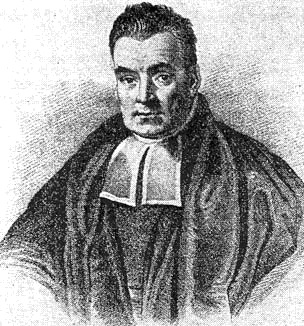
\includegraphics[scale=0.75]{figures/Thomas_Bayes.jpeg}
    \caption{Thomas Joshua Bayes (1702-1761)}
    \label{fig:my_label2}
\end{figure}


Seu trabalho com as probabilidades foi reunido em um ensaio
publicado após a sua morte (em 1763) no livro Philosophical
Transactions of the Royal Society of London. O ensaio Essay
Towards Solving a Problem in the Doctrine of Chances relatou,
entre outras importantes descobertas de Bayes, o famoso Teorema de
Bayes.

\newpage
\subsection{ O Que é o Teorema de Bayes}

O teorema de Bayes é usado na inferência estatística para
atualizar estimativas da probabilidade de que diferentes hipóteses
sejam verdadeiras, baseado nas observações e no conhecimento de
como essas observações se relacionam com as hipóteses.\vskip0.3cm

Este teorema é uma das pedras angulares da estatística das
probabilidades combinadas, e é largamente utilizada em áreas a
primeira vista pouco relacionadas, como Medicina e
Informática.\vskip0.3cm

Na primeira, o paradigma embasado em evidências é todo construído
em cima do teorema de Bayes. Baseado na experiência acumulada de
exames e testes para tentar diagnosticar uma doença, o médico
enquadra seus pacientes e pode estimar qual a probabilidade de que
uma dada doença esteja se manifestando. Ou seja, dada uma
probabilidade inicial (por exemplo, o paciente é fumante) e
aplicado um exame em que, se sabe, há uma probabilidade de
falsos-positivos e falso-negativos (por exemplo, uma biópsia de
pulmão), o médico sabe qual a probabilidade resultante daquele
paciente ter a doença (por exemplo, câncer de pulmão).\vskip0.3cm

Na informática, muitos dos sistemas de classificação automática
são baseados no teorema de Bayes. Inicialmente o sistema é
treinado, aceitando entradas de humanos que dizem que uma dada
entrada pertencem a determinado grupo. Com o tempo, o sistema
acumula um grande banco dessas informações e, aplicando o teorema
de Bayes, consegue estimar a probabilidade de cada novo dado de
pertencer a cada grupo já classificado.\vskip0.3cm

%\newpage
\subsection{Definição do Teorema}

Seja $B_1,B_2,\dots,B_k$ uma partição do espaço amostral $S$ e seja $A$ um evento qualquer.
Então, para cada $i$, vale:

\begin{equation}\label{bayes}
P(B_i\mid A)=
\frac{P(A\mid B_i)\,P(B_i)}
{\sum_{j=1}^{k}P(A\mid B_j)\,P(B_j)}.
\end{equation}

Esse resultado é conhecido como \textbf{Teorema de Bayes} e constitui a base da chamada
\textbf{Estatística Bayesiana}. È também denominado fórmula da probabilidade das causas (ou dos antededentes). Desde que os $B_{i}$ constituam uma partição do espaço amostral um, e somente um, dos eventos $B_{i}$ ocorrerá.

\newpage
A ídéia expressa no Teorema da Bayes deu origem a uma nova, moderna e alternativa maneira de se pensar a Estatística, gerando a chamada \textbf{Estatística Bayesiana}. 


\subsection{Árvores de Probabilidades}

A construção de uma \textbf{árvore de probabilidades}, também chamada de
\textbf{diagrama de árvore}, é uma ferramenta fundamental na solução de problemas
probabilísticos que envolvem \textbf{duas ou mais etapas sucessivas}. \vskip0.3cm

Esse tipo de representação é especialmente útil quando um experimento ocorre de
forma \textbf{sequencial}, isto é, quando o resultado de uma etapa influencia as
probabilidades da etapa seguinte. Assim, árvores de probabilidade permitem
organizar visualmente os possíveis caminhos de um experimento e calcular
probabilidades de eventos compostos de maneira sistemática.


\bigskip

\subsubsection{Estrutura Matemática}

Considere dois eventos $A$ e $B$. A probabilidade de ocorrência conjunta desses
eventos é dada pela regra do produto:

\begin{equation}
P(A \cap B) = P(A)\cdot P(B \mid A),
\end{equation}

onde $P(B \mid A)$ representa a \textbf{probabilidade condicional} de $B$
ocorrer dado que $A$ já ocorreu.

De forma geral, para um experimento com $n$ etapas sequenciais, a probabilidade
de um caminho completo é obtida multiplicando-se as probabilidades condicionais:

\begin{equation}
P(E_1 \cap E_2 \cap \dots \cap E_n)
=
P(E_1)\cdot P(E_2\mid E_1)\cdot\dots\cdot P(E_n\mid E_1\cap\dots\cap E_{n-1}).
\end{equation}



\subsubsection{Exemplo 1: Sorteio Sequencial}

Suponha uma urna contendo $5$ bolas, sendo $3$ verdes e $2$ vermelhas.
Retiram-se duas bolas \textbf{sem reposição}.

\begin{itemize}
\item Evento $V_1$: primeira bola verde.
\item Evento $V_2$: segunda bola verde.
\end{itemize}

A probabilidade da primeira bola ser verde é:

\begin{equation}
P(V_1)=\frac{3}{5}.
\end{equation}

Como não há reposição, restam $4$ bolas, sendo $2$ verdes. Assim:

\begin{equation}
P(V_2\mid V_1)=\frac{2}{4}.
\end{equation}

Logo, a probabilidade de retirar duas bolas verdes é:

\begin{equation}
P(V_1\cap V_2)=P(V_1)\cdot P(V_2\mid V_1)
=\frac{3}{5}\cdot\frac{2}{4}
=\frac{3}{10}.
\end{equation}

\bigskip

\subsubsection{Exemplo 2: Aplicação em Tomada de Decisão Pública}

Considere um sistema de monitoramento ambiental que detecta risco de desmatamento.

\begin{itemize}
\item Evento $D$: há desmatamento real na região.
\item Evento $S$: o sensor emite alerta positivo.
\end{itemize}

Suponha:

\begin{equation}
P(D)=0.20,
\qquad
P(S\mid D)=0.90,
\qquad
P(S\mid D^c)=0.10.
\end{equation}

A probabilidade de o sensor emitir alerta e realmente haver desmatamento é:

\begin{equation}
P(D\cap S)=P(D)\cdot P(S\mid D)
=0.20\cdot0.90
=0.18.
\end{equation}

Esse tipo de análise é essencial para políticas públicas baseadas em dados,
pois permite quantificar incertezas e aprimorar decisões estratégicas na gestão
ambiental.

\newpage
\section{Eventos Independentes}

Em Probabilidade, um dos conceitos mais importantes é o de \textbf{independência entre eventos}. \vskip0.3cm

Dois eventos $A$ e $B$ são ditos \textbf{independentes} quando a ocorrência de
um deles \textbf{não influencia} a chance de ocorrência do outro. Em outras palavras, saber que $A$ ocorreu não altera a probabilidade de $B$,
isto é,

\begin{equation}
P(B\mid A)=P(B).
\end{equation}

De forma equivalente, dois eventos são independentes se satisfazem a regra:

\begin{equation}
P(A\cap B)=P(A)\cdot P(B).
\end{equation}

Essa propriedade indica que a probabilidade de ambos ocorrerem simultaneamente
é simplesmente o produto das probabilidades individuais.



\subsection*{Exemplo 1: Lançamento de Moeda e Dado}

Considere o experimento composto:

\begin{itemize}
\item Lançar uma moeda.
\item Lançar um dado de seis faces.
\end{itemize}

Defina os eventos:

\begin{itemize}
\item $A$: sair \textbf{cara} na moeda.
\item $B$: sair um número \textbf{par} no dado.
\end{itemize}

Temos:

\[
P(A)=\frac{1}{2},
\qquad
P(B)=\frac{3}{6}=\frac{1}{2}.
\]

Como os experimentos não interferem entre si, os eventos são independentes.
Logo,

\begin{equation}
P(A\cap B)=P(A)\cdot P(B)
=\frac{1}{2}\cdot\frac{1}{2}
=\frac{1}{4}.
\end{equation}

Portanto, a probabilidade de sair \textbf{cara} e um número \textbf{par} é $0,25$.


\subsection*{Exemplo 2: Aplicação em Gestão Pública}

Suponha que, em um determinado município do Pará:

\begin{itemize}
\item $A$: ocorrer chuva intensa em um dia.
\item $B$: ocorrer um acidente de trânsito urbano no mesmo dia.
\end{itemize}

Se estudos indicam que esses eventos são estatisticamente independentes, então:

\[
P(A)=0.30,
\qquad
P(B)=0.10.
\]

Logo, a probabilidade de ocorrerem simultaneamente é:

\begin{equation}
P(A\cap B)=0.30\cdot0.10=0.03.
\end{equation}

Assim, existe uma chance de apenas $3\%$ de que, no mesmo dia, haja
chuva intensa e acidente urbano.



\subsection*{Independência de Três Eventos}

Considere agora três eventos $A$, $B$ e $C$.

Dizemos que eles são \textbf{mutuamente independentes} quando todas as combinações
possíveis também são independentes, ou seja:

\begin{equation}
P(A\cap B)=P(A)P(B),
\qquad
P(A\cap C)=P(A)P(C),
\qquad
P(B\cap C)=P(B)P(C),
\end{equation}

e adicionalmente:

\begin{equation}
P(A\cap B\cap C)=P(A)P(B)P(C).
\end{equation}


\subsection*{Exemplo 3: Três Sensores Independentes}

Imagine três sensores ambientais que monitoram queimadas na floresta:

\begin{itemize}
\item $A$: sensor 1 detecta foco.
\item $B$: sensor 2 detecta foco.
\item $C$: sensor 3 detecta foco.
\end{itemize}

Suponha que:

\[
P(A)=0.20,
\qquad
P(B)=0.30,
\qquad
P(C)=0.10.
\]

Se os sensores funcionam de forma independente, então:

\begin{equation}
P(A\cap B\cap C)
=0.20\cdot0.30\cdot0.10
=0.006.
\end{equation}

Logo, a chance de os três sensores detectarem simultaneamente um foco é de
apenas $0,6\%$.

\bigskip

\subsection*{Generalização: Independência Mútua}

De maneira geral, um conjunto de eventos $A_1,A_2,\dots,A_n$ é dito
\textbf{mutuamente independente} se, para qualquer subconjunto com $k\geq 2$
eventos, vale:

\begin{equation}
P(A_{i_1}\cap A_{i_2}\cap\cdots\cap A_{i_k})
=
P(A_{i_1})P(A_{i_2})\cdots P(A_{i_k}).
\end{equation}

\bigskip

\subsection*{Observação Importante}

É essencial destacar que:

\begin{quote}
Independência dois a dois \textbf{não garante} independência mútua.
\end{quote}

Ou seja, pode ocorrer que todos os pares de eventos sejam independentes,
mas o conjunto completo não seja. Assim, a independência é uma hipótese forte, amplamente utilizada em modelos estatísticos, inferência e simulações computacionais, pois simplifica cálculos
e permite compreender sistemas complexos com maior clareza.


\begin{figure}[H]
\centering
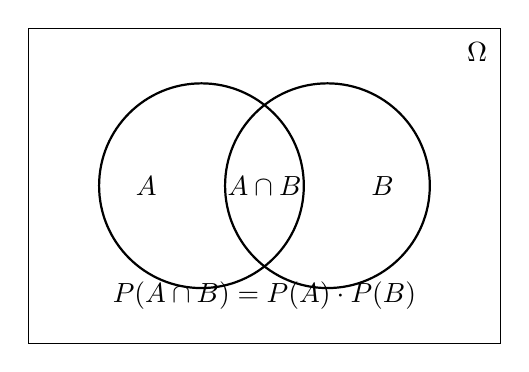
\begin{tikzpicture}[scale=1.0]

% Universo
\draw (0,0) rectangle (6,4);
\node at (5.7,3.7) {$\Omega$};

% Conjuntos A e B
\draw[thick] (2.2,2) circle (1.3);
\draw[thick] (3.8,2) circle (1.3);

% Labels
\node at (1.5,2) {$A$};
\node at (4.5,2) {$B$};

% Interseção
\node at (3,2) {$A\cap B$};

% Probabilidade
\node at (3,0.6)
{$P(A\cap B)=P(A)\cdot P(B)$};

\end{tikzpicture}
\caption{Diagrama de Venn ilustrando dois eventos independentes.}
\label{fig:venn_independencia}
\end{figure}


%----------------------------------------------------------------------------------------%
%------------------------- var ----------------------------------------------------------%
\newpage
\section{Variáveis Aleatórias Unidimensionais}
\subsection{Introdução}


Em muitos experimentos aleatórios, o espaço amostral $\Omega$ é formado por resultados que não são, necessariamente, números.
Por exemplo, no lançamento de duas moedas, o espaço amostral é dado por:

\[
\Omega=\{CC,\,CK,\,KC,\,KK\},
\]

onde $C$ representa ``cara'' e $K$ representa ``coroa''.

\vskip0.3cm

Em diversas situações, entretanto, não estamos interessados na sequência exata obtida, mas sim em alguma característica numérica associada ao resultado.
Por exemplo:

\begin{itemize}
    \item ao lançar três moedas, pode-se desejar apenas o número de caras obtidas;
    \item ao lançar uma moeda repetidamente até aparecer cara, pode-se estar interessado no número de lançamentos necessários.
\end{itemize}

\vskip0.3cm

Assim, surge a necessidade de associar a cada resultado do espaço amostral um valor numérico real.
Esse tipo de associação conduz ao conceito fundamental de \textbf{variável aleatória}.

\subsection{Definição}

Seja $\Omega$ o espaço amostral de um experimento aleatório.
Uma função

\[
X:\Omega \longrightarrow \mathbb{R},
\]

que associa a cada resultado $s\in\Omega$ um número real $X(s)$, é denominada uma
\textbf{variável aleatória}.

\vskip0.3cm

O conjunto de todos os valores possíveis assumidos por $X$ é chamado de
\textbf{imagem} (ou conjunto de valores) da variável aleatória, e é denotado por:

\[
X(\Omega)=\{x\in\mathbb{R}\;:\; X(s)=x,\; s\in\Omega\}.
\]

\vskip0.3cm

Em geral, utilizamos letras maiúsculas ($X,Y,Z,\dots$) para representar variáveis aleatórias e letras minúsculas ($x,y,z,\dots$) para representar valores possíveis dessas variáveis.


\subsection{Exemplo: Número de caras em três lançamentos}

Considere o experimento de lançar três moedas equilibradas. O espaço amostral é composto por todas as sequências possíveis de caras e coroas.  \vskip0.3cm

Defina a variável aleatória $X$ como:

\[
X(s)=\text{número de caras obtidas na sequência } s.
\]

Logo, o conjunto de valores possíveis é:

\[
X(\Omega)=\{0,1,2,3\}.
\]

A tabela a seguir apresenta os resultados possíveis e os respectivos valores de $X$, durante uma jogada de lancamento de dados:

\begin{table}[H]
\centering
\caption{Variável aleatória $X$: número de caras em três lançamentos.}
\begin{tabular}{c|cccccccc}
\hline\hline
$\Omega$     & KKK & CKK & KCK & KKC & CCK & CKC & KCC & CCC\\
\hline
$X(s)$       & 0   & 1   & 1   & 1   & 2   & 2   & 2   & 3\\
\hline\hline
\end{tabular}
\end{table}

\vskip0.3cm

Note que, sobre o mesmo espaço amostral, poderíamos definir diversas outras variáveis aleatórias, como o número de coroas, ou a diferença entre caras e coroas.

\newpage
\section{Variável Aleatória Discreta}
\subsection{Definição}

Uma variável aleatória $X$ é chamada de \textbf{discreta} quando assume valores em um conjunto finito ou infinito enumerável, isto é,

\[
X(\Omega)=\{x_1,x_2,x_3,\dots\}.
\]

\subsection{Função de Probabilidade}

Se $X$ é uma variável aleatória discreta, define-se sua
\textbf{função de probabilidade} como:

\[
f(x_i)=P(X=x_i),
\]

onde $x_i$ é um valor possível de $X$. Essa função satisfaz as propriedades:

\[
f(x_i)\geq 0,\quad \forall i,
\]

\[
\sum_{i} f(x_i)=1.
\]

\subsection{Exemplo: Duas moedas}

Considere o lançamento de duas moedas e seja $X$ o número de caras obtidas.

\[
\Omega=\{CC,CK,KC,KK\}.
\]

\begin{table}[H]
\centering
\caption{Valores possíveis da variável aleatória $X$.}
\begin{tabular}{c|cccc}
\hline\hline
Resultado & CC & CK & KC & KK\\
\hline
$X(s)$    & 2  & 1  & 1  & 0\\
\hline\hline
\end{tabular}
\end{table}

Assim, a função de probabilidade é:

\begin{table}[H]
\centering
\caption{Distribuição de probabilidade de $X$.}
\begin{tabular}{c|ccc}
\hline\hline
$x$      & 0   & 1   & 2\\
\hline
$f(x)$   & 1/4 & 1/2 & 1/4\\
\hline\hline
\end{tabular}
\end{table}


\subsection{Função de Distribuição Acumulada (FDA)}

A função de distribuição acumulada de $X$ é definida por:

\[
F(x)=P(X\leq x).
\]

No caso discreto, temos:

\[
F(x)=\sum_{x_i\leq x} f(x_i).
\]



\subsection{Esperança Matemática}

Se $X$ assume valores $x_1,x_2,\dots$, então a esperança de $X$ é:

\[
E(X)=\sum_i x_i\,P(X=x_i).
\]


\subsection{Variância}

A variância de $X$ mede a dispersão dos valores em torno da média:

\[
V(X)=E(X^2)-[E(X)]^2.
\]

onde

\[
E(X^2)=\sum_i x_i^2\,P(X=x_i).
\]



%----------------------------------------------------------------------------------%



\newpage
%%%%%%%%%%%%%%%%%%%%%%%%%%%%%%%%%%%%%%%%%%%%%%%%%%%%%%%%%%%%%%%%%%%%%%%%%%%%%%%%%%%%

\section{Variáveis Aleatórias Contínuas (V.A.C.)}

De modo geral, muitas grandezas observadas na natureza não são obtidas por contagem, mas sim por \textbf{mensuração}.
Por exemplo:

\begin{itemize}
    \item Peso de um Paciente,
    \item tempo de Espera em um Atendimento,
    \item Temperatura Ambiente,
    \item Nível de Voltagem em um Circuito,
    \item Concentração de um Poluente no Ar.
\end{itemize}

Essas quantidades podem assumir infinitos valores dentro de um intervalo real, sendo mais adequadamente descritas como
\textbf{variáveis aleatórias contínuas}. \vskip0.3cm

Por outro lado, variáveis associadas a \textbf{contagens} (como número de veículos em uma via ou quantidade de atendimentos em um hospital) são tipicamente modeladas como variáveis aleatórias discretas. \vskip0.3cm

Em alguns casos, a distinção depende do nível de precisão da medida.
Por exemplo, o comprimento de uma peça é uma variável contínua, mas se for arredondado para duas casas decimais pode ser tratado como discreto.

\subsection{Definição}

Seja $\Omega$ o espaço amostral de um experimento aleatório.
Uma variável aleatória $X$ é dita \textbf{contínua} se seu conjunto de valores possíveis $X(\Omega)$ é infinito não enumerável, isto é, se assume valores em um intervalo (ou união de intervalos) da reta real.

\subsection{Função Densidade de Probabilidade}

Uma variável aleatória contínua $X$ é caracterizada por uma função
$f(x)$, chamada de \textbf{função densidade de probabilidade (fdp)}, que satisfaz:

\begin{enumerate}
    \item Não negatividade:
    \[
    f(x)\geq 0,\quad \forall x\in\mathbb{R};
    \]

    \item Normalização:
    \[
    \int_{-\infty}^{+\infty} f(x)\,dx = 1.
    \]
\end{enumerate}

\vskip0.3cm

A probabilidade de $X$ assumir valores dentro de um intervalo $(a,b)$ é dada por:

\[
P(a<X<b)=\int_a^b f(x)\,dx.
\]

\vskip0.3cm

Um ponto fundamental é que, para variáveis contínuas,

\[
P(X=x)=0.
\]

Ou seja, probabilidades são sempre associadas a intervalos, e não a valores isolados.


\subsection{Exemplo: Tempo de vida de uma lâmpada}

Suponha que o tempo de duração (em anos) de uma lâmpada seja uma variável aleatória contínua com densidade:

\[
f(x)=
\begin{cases}
2e^{-2x}, & x\geq 0,\\
0, & \text{caso contrário}.
\end{cases}
\]

Essa é uma distribuição exponencial, frequentemente utilizada em modelos de confiabilidade e tempo de falha.


\subsection{Função Distribuição Acumulada}

A função de distribuição acumulada (FDA) de uma variável contínua $X$ é definida por:

\[
F(x)=P(X\leq x).
\]

No caso contínuo, temos:

\[
F(x)=\int_{-\infty}^{x} f(s)\,ds.
\]



\subsection{Exemplo: Construção de uma FDA}

Considere a densidade:

\[
f(x)=
\begin{cases}
\frac{1}{2}x, & 0<x<2,\\
0, & \text{caso contrário}.
\end{cases}
\]

A FDA é obtida por integração:

\[
F(x)=\int_0^x \frac{1}{2}s\,ds=\frac{1}{4}x^2,\quad 0\leq x\leq 2.
\]

Portanto,

\[
F(x)=
\begin{cases}
0, & x<0,\\[0.2cm]
\frac{1}{4}x^2, & 0\leq x\leq 2,\\[0.2cm]
1, & x>2.
\end{cases}
\]



\subsection{Esperança Matemática}

Se $X$ é uma variável aleatória contínua com densidade $f(x)$, então sua esperança é:

\[
\boxed{
E(X)=\int_{-\infty}^{+\infty} x f(x)\,dx.
}
\]

Esse valor representa a média teórica da distribuição.



%---------------------------------------------------------------------------%
\subsection{Variância}

A variância é uma das medidas mais importantes em Probabilidade e Estatística,
pois quantifica o grau de dispersão dos valores assumidos por uma variável
aleatória em torno de sua média. \vskip0.3cm

Seja $X$ uma variável aleatória contínua com esperança matemática (média)

\[
\mu = E(X).
\]

A variância de $X$, denotada por $V(X)$ ou $\mathrm{Var}(X)$,
é definida como o valor esperado do quadrado do desvio de $X$ em relação à média:

\begin{equation}
V(X)=E\big[(X-\mu)^2\big].
\end{equation}

\vskip0.3cm

Essa definição expressa que a variância mede o quanto os valores de $X$
se afastam, em média, do valor central $\mu$.


\subsubsection{Demonstração da Fórmula Alternativa}

A expressão acima pode ser desenvolvida algebricamente.
Começamos expandindo o termo quadrático:

\[
(X-\mu)^2 = X^2 -2\mu X +\mu^2.
\]

Aplicando o operador esperança em ambos os lados, obtemos:

\[
V(X)=E(X^2 -2\mu X +\mu^2).
\]

Pela linearidade da esperança, temos:

\[
V(X)=E(X^2)-2\mu E(X)+E(\mu^2).
\]

Agora, note que $\mu$ é uma constante, pois $\mu=E(X)$.
Logo:

\[
E(\mu^2)=\mu^2.
\]

Além disso, como $E(X)=\mu$, segue que:

\[
-2\mu E(X)=-2\mu\cdot \mu=-2\mu^2.
\]

Substituindo esses resultados na expressão anterior:

\[
V(X)=E(X^2)-2\mu^2+\mu^2.
\]

Portanto:

\[
V(X)=E(X^2)-\mu^2.
\]

Finalmente, como $\mu=E(X)$, concluímos que:

\begin{equation}
\boxed{
V(X)=E(X^2)-[E(X)]^2.
}
\end{equation}


\newpage
\subsubsection{Expressão Integral para Variáveis Contínuas}

Se $X$ é contínua e possui função densidade de probabilidade $f(x)$,
então o segundo momento de $X$ é dado por:

\[
\boxed{
E(X^2)=\int_{-\infty}^{+\infty}x^2 f(x)\,dx.
}
\]

Assim, a variância pode ser escrita como:

\[
V(X)=
\int_{-\infty}^{+\infty}x^2 f(x)\,dx
-
\left(
\int_{-\infty}^{+\infty}x f(x)\,dx
\right)^2.
\]

\vskip0.3cm

Essa forma mostra que a variância depende do segundo momento de $X$ e do quadrado de sua média.


\subsection{Exemplo Completo}

Considere a densidade:

\[
f(x)=
\begin{cases}
\frac{1}{8}x^2, & 0<x<2,\\
0, & \text{caso contrário}.
\end{cases}
\]

\textbf{(i) Esperança}

\[
E(X)=\int_0^2 x\cdot \frac{1}{8}x^2\,dx
=\frac{1}{8}\int_0^2 x^3\,dx
=\frac{1}{8}\cdot\frac{2^4}{4}
=1.
\]

\textbf{(ii) Segundo momento}

\[
E(X^2)=\int_0^2 x^2\cdot \frac{1}{8}x^2\,dx
=\frac{1}{8}\int_0^2 x^4\,dx
=\frac{1}{8}\cdot\frac{2^5}{5}
=\frac{4}{5}.
\]

\textbf{(iii) Variância}

\[
V(X)=\frac{4}{5}-1^2=\frac{-1}{5}.
\]

(Portanto, este exemplo mostra que uma escolha inadequada de densidade pode gerar inconsistências, reforçando a necessidade de verificar a normalização.)


\subsection{Exercício Proposto}

Seja $X$ uma variável aleatória contínua com densidade:

\[
f(x)=
\begin{cases}
cx^2, & 0<x<3,\\
0, & \text{caso contrário}.
\end{cases}
\]

\begin{enumerate}
    \item Determine a constante $c$.
    \item Obtenha a função distribuição acumulada $F(x)$.
    \item Calcule $P(1<X\leq 2)$.
    \item Determine $E(X)$ e $V(X)$.
\end{enumerate}


%------------------------------------------------------------------------------------------%
\subsection{Propriedades da Esperança e Variância}

A esperança matemática é um operador fundamental na Teoria da Probabilidade,
pois permite determinar o valor médio esperado de uma variável aleatória.
Além disso, ela possui propriedades algébricas essenciais que simplificam
cálculos em diversos modelos estatísticos. \vskip0.3cm

Sejam $X$ e $Y$ variáveis aleatórias com esperança finita e seja $k\in\mathbb{R}$
uma constante real. Então, valem as seguintes propriedades.

\subsubsection{Propriedade 1: Esperança de uma constante}

\begin{equation}
E(k)=k.
\end{equation}

\textbf{Demonstração:} Se $k$ é uma constante, então a variável aleatória assume sempre o mesmo valor. Pela definição da esperança para variáveis contínuas:

\[
E(k)=\int_{-\infty}^{+\infty} k\, f(x)\,dx.
\]

Como $k$ é constante, pode ser colocado fora da integral:

\[
E(k)=k\int_{-\infty}^{+\infty} f(x)\,dx.
\]

Mas toda função densidade satisfaz:

\[
\int_{-\infty}^{+\infty} f(x)\,dx=1.
\]

Logo:

\[
E(k)= k \times 1 = k.
\]

\subsubsection{Propriedade 2: Esperança de um múltiplo constante}

\begin{equation}
E(kX)=kE(X).
\end{equation}

\textbf{Demonstração:} Pela definição:

\[
E(kX)=\int_{-\infty}^{+\infty} (kx)\, f(x)\,dx.
\]

Colocando $k$ em evidência:

\[
E(kX)=k\int_{-\infty}^{+\infty} x f(x)\,dx.
\]

Mas o termo integral é exatamente $E(X)$:

\[
E(kX)=kE(X).
\]

\subsubsection{Propriedade 3: Esperança de uma soma com constante}

\begin{equation}
E(X+k)=E(X)+k.
\end{equation}

\textbf{Demonstração:}

Temos:

\[
E(X+k)=\int_{-\infty}^{+\infty} (x+k)\, f(x)\,dx.
\]

Separando a integral:

\[
E(X+k)=\int_{-\infty}^{+\infty} x f(x)\,dx
+\int_{-\infty}^{+\infty} k f(x)\,dx.
\]

O primeiro termo é $E(X)$ e o segundo é $k$, pois:

\[
\int_{-\infty}^{+\infty} f(x)\,dx=1.
\]

Portanto:

\[
E(X+k)=E(X)+k.
\]


\subsubsection{Propriedade 4: Linearidade da esperança}

\begin{equation}
E(X\pm Y)=E(X)\pm E(Y).
\end{equation}

\textbf{Demonstração:} Considerando a esperança de uma soma:

\[
E(X+Y)=\int_{-\infty}^{+\infty}(x+y)\,f_{X,Y}(x,y)\,dx\,dy.
\]

Distribuindo:

\[
E(X+Y)=\int\int x f_{X,Y}(x,y)\,dx\,dy
+\int\int y f_{X,Y}(x,y)\,dx\,dy.
\]

O primeiro termo corresponde a $E(X)$ e o segundo a $E(Y)$:

\[
E(X+Y)=E(X)+E(Y).
\]

O caso da diferença é análogo:

\[
E(X-Y)=E(X)-E(Y).
\]


\subsubsection{Propriedade 5: Esperança do produto de variáveis independentes}

Se $X$ e $Y$ são independentes, então:

\begin{equation}
E(XY)=E(X)\,E(Y).
\end{equation}

\textbf{Demonstração:} Pela definição:

\[
E(XY)=\int_{-\infty}^{+\infty}\int_{-\infty}^{+\infty}
xy\,f_{X,Y}(x,y)\,dx\,dy.
\]

Se $X$ e $Y$ são independentes, então:

\[
f_{X,Y}(x,y)=f_X(x)\,f_Y(y).
\]

Logo:

\[
E(XY)=\int\int xy\,f_X(x)f_Y(y)\,dx\,dy.
\]

Separando os termos:

\[
E(XY)=
\left(\int_{-\infty}^{+\infty} x f_X(x)\,dx\right)
\left(\int_{-\infty}^{+\infty} y f_Y(y)\,dy\right).
\]

Mas:

\[
\int x f_X(x)\,dx=E(X),
\qquad
\int y f_Y(y)\,dy=E(Y).
\]

Portanto:

\[
E(XY)=E(X)\,E(Y).
\]
\vskip0.3cm

Essas propriedades mostram que a esperança é um operador linear e que,
sob independência, o valor esperado do produto se decompõe no produto das esperanças,
um resultado central em Estatística e Inferência.

\subsubsection{Propriedades da Variância}

Além da esperança, outra medida fundamental é a variância, que quantifica
o grau de dispersão dos valores de uma variável aleatória em torno de sua média.

\vskip0.3cm

Recordemos que, para uma variável aleatória contínua $X$, a variância é definida por:

\[
V(X)=E\big[(X-E(X))^2\big].
\]

Uma forma equivalente muito utilizada é:

\[
V(X)=E(X^2)-[E(X)]^2.
\]

A seguir apresentamos algumas propriedades importantes.

\subsubsection{Propriedade 1: Variância de uma constante}

\begin{equation}
V(k)=0.
\end{equation}

\textbf{Demonstração:}

Se $k$ é constante, então:

\[
E(k)=k.
\]

Logo:

\[
V(k)=E\big[(k-E(k))^2\big].
\]

Mas como $E(k)=k$, temos:

\[
V(k)=E\big[(k-k)^2\big]=E(0)=0.
\]

Portanto, uma constante não apresenta dispersão.



\subsubsection{Propriedade 2: Variância de um múltiplo constante}

\begin{equation}
V(kX)=k^2V(X).
\end{equation}

\textbf{Demonstração:} Pela definição:

\[
V(kX)=E\big[(kX-E(kX))^2\big].
\]

Usando a propriedade da esperança:

\[
E(kX)=kE(X).
\]

Substituindo:

\[
V(kX)=E\big[(kX-kE(X))^2\big].
\]

Fatorando $k$:

\[
V(kX)=E\big[k^2(X-E(X))^2\big].
\]

Como $k^2$ é constante:

\[
V(kX)=k^2E\big[(X-E(X))^2\big].
\]

Mas o termo interno é a variância de $X$:

\[
V(kX)=k^2V(X).
\]


\subsubsection{Propriedade 3: Variância de uma soma com constante}

\begin{equation}
V(X+k)=V(X).
\end{equation}

\textbf{Demonstração:} Temos:

\[
V(X+k)=E\big[(X+k-E(X+k))^2\big].
\]

Pela propriedade da esperança:

\[
E(X+k)=E(X)+k.
\]

Logo:

\[
V(X+k)=E\big[(X+k-(E(X)+k))^2\big].
\]

Cancelando os termos $k$:

\[
V(X+k)=E\big[(X-E(X))^2\big].
\]

Portanto:

\[
V(X+k)=V(X).
\]

Isso mostra que adicionar uma constante desloca a variável,
mas não altera sua dispersão.



\subsubsection{Propriedade 4: Variância da soma de duas variáveis}

Para quaisquer variáveis aleatórias $X$ e $Y$:

\begin{equation}
V(X+Y)=V(X)+V(Y)+2\,\mathrm{Cov}(X,Y),
\end{equation}

onde $\mathrm{Cov}(X,Y)$ é a covariância definida por:

\[
\mathrm{Cov}(X,Y)=E(XY)-E(X)E(Y).
\]

\textbf{Demonstração:} Pela definição:

\[
V(X+Y)=E\big[(X+Y-E(X+Y))^2\big].
\]

Como:

\[
E(X+Y)=E(X)+E(Y),
\]

então:

\[
V(X+Y)=E\big[(X+Y-E(X)-E(Y))^2\big].
\]

Reescrevendo:

\[
V(X+Y)=E\big[((X-E(X))+(Y-E(Y)))^2\big].
\]

Expandindo o quadrado:

\[
V(X+Y)=E\big[(X-E(X))^2+(Y-E(Y))^2
+2(X-E(X))(Y-E(Y))\big].
\]

Aplicando linearidade da esperança:

\[
V(X+Y)=E[(X-E(X))^2]+E[(Y-E(Y))^2]
+2E[(X-E(X))(Y-E(Y))].
\]

Reconhecendo:

\[
E[(X-E(X))^2]=V(X),
\qquad
E[(Y-E(Y))^2]=V(Y),
\]

e o termo cruzado é a covariância:

\[
E[(X-E(X))(Y-E(Y))]=\mathrm{Cov}(X,Y).
\]

Logo:

\[
V(X+Y)=V(X)+V(Y)+2\,\mathrm{Cov}(X,Y).
\]



\subsubsection{Caso Especial: Soma de variáveis independentes}

Se $X$ e $Y$ são independentes, então:

\[
\mathrm{Cov}(X,Y)=0.
\]

Assim:

\begin{equation}
V(X+Y)=V(X)+V(Y).
\end{equation}

A variância de uma soma de variáveis independentes é igual à soma das variâncias,
um resultado central em Estatística e Probabilidade.
%------------------------------------------------------------------------------------------%




%------------------------------------------------------------------------------------------%
\newpage
\section{Principais Distribuições de Probabilidade}
 

Uma distribuição de probabilidade é um modelo matemático que relaciona um certo valor da variável aleatória em estudo com a sua probabilidade de ocorrência. De conformidade com a natureza da variável aleatória, a distribuição pode ser classificada em discreta ou contínua.
 
\subsection{Distribuição Binomial}

Os princípios básicos da distribuição binomial foram desenvolvidos pelo matemático suíço durante o século XVII chamado \textbf{Jakob Bernoulli}, que fez muitas contribuições à teoria da probabilidade. Foi o autor do que é geralmente conhecido como o primeiro livro dedicado à probabilidade, publicado em 1713.

\vspace{-0.3cm}
\begin{figure}
    \centering
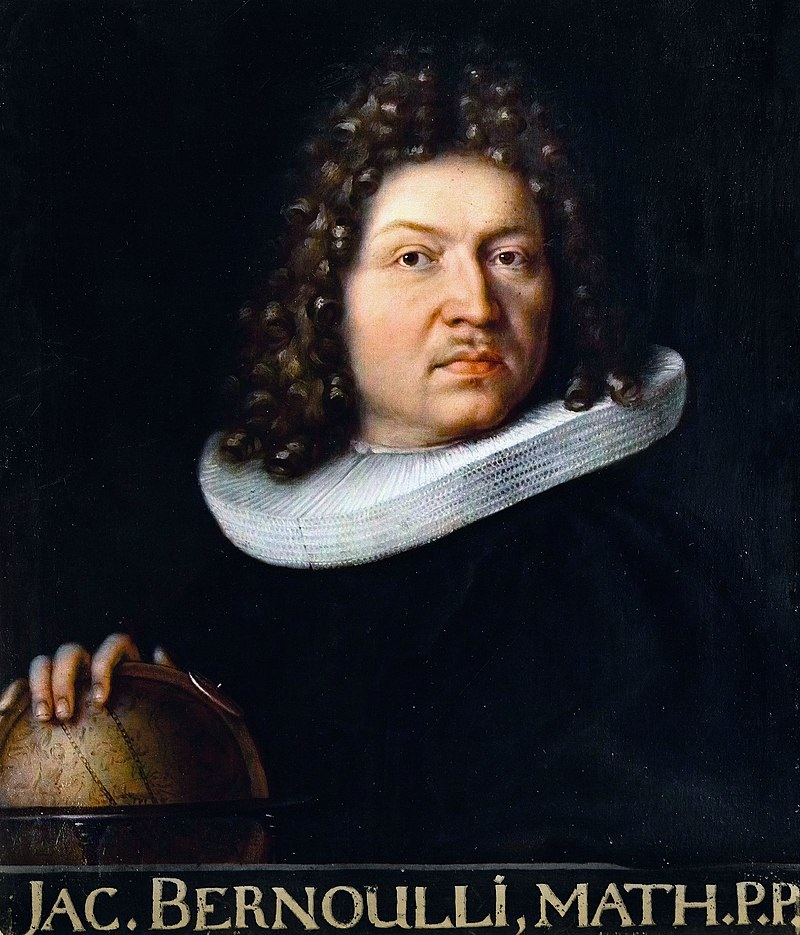
\includegraphics[scale=0.25]{figures/Jakob_Bernoulli.jpeg}
    \caption{Jakob Bernoulli(1654-1705)}
    \label{fig:my_label4}
\end{figure}

Jakob nasceu em Basel na Suiça, estudou Teologia, Matemática e Astronomia na Universidade de Basel. Entre os nomes associados à instituição estão os de \textbf{Leonhard Euler}, \textbf{Friedrich Nietzsche}, e \textbf{Eugen Huber} um jurista famoso e criador do Código Civil Suiço. \vskip0.3cm



\newpage
Em homenagem a Jakob, os ensaios utilizando probabilidade binomial, na maioria das vezes são denominados \textbf{Ensaios de Bernoulli}, e uma sequência desse tipo de ensaios é denominado de \textbf{Processo de Bernoulli} 
\vskip0.3cm


A distribuição Binomial dá a probabilidade de deterninado desfecho ocorrer em determinado número de ensaios independentes. \vskip0.3cm


A distribuição Binomial é uma distribuição discreta, cuja função de probabilidade é:
 
\begin{equation}
f(y) = C_{n}^{y}p^{y}q^{n-y}
\end{equation}
 
Sendo: \vskip0.3cm

\begin{itemize}
\item $p$ = probabilidade de realização do acontecimento favorável; 
\item  $q$ = probabilidade de ralização do acontecimento contrário;  
\item $y$ = número de vezes que se realiza o acontecimento favorável;  
\item $n$ = número de tentativas; 
\item $C_{n}^{y}$ = números de combinações de n elementos, tomados y a y; 
\end{itemize} 

\newpage
\subsection{Distribuição de Poisson}

A distribuição de Poisson tem este nome em homenagem ao metemático, Astrônomo e físico francês \textbf{Simeon Denis Poisson}. Com característica próxima a Binomial, a distribuição de Poisson é uma distribuição descontínua, aplicável quando o resultado é o número de vezes que determinado evento ocorre. 


\vspace{-0.3cm}
\begin{figure}
    \centering
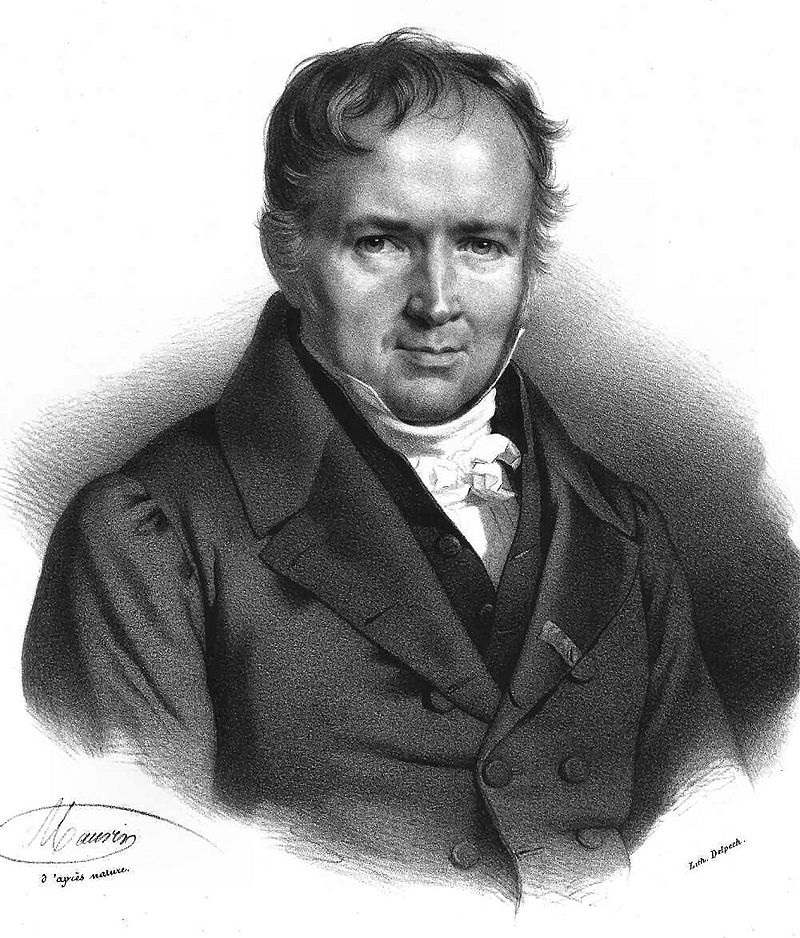
\includegraphics[scale=0.25]{figures/Simeon_Poisson.jpeg}
    \caption{Simeon Denis Poisson(1781-1840)}
    \label{fig:my_label4}
\end{figure}


Poisson recebeu dois prêmios importantes da época:

\begin{itemize}
    \item \textbf{Prêmio Lalande (1810):} Membro da Academia Americana de Artes e Ciências;
    \item \textbf{Medalha Copley (1832):} (For his work entitled, Nouvelle Theorie de lAction Capillaire., 1832)
\end{itemize}

O Prêmio Lalande foi uma condecoração científica em Astronomia, concedida de 1902 a 1970 pela Académie des Sciences. O prêmio homenageia o astrônomo Jérôme Lalande, estabelecido pelo próprio em 1801. Após 1970 foi combinado com o prêmio da fundação Benjamin Valz, concedido até 1996.\vskip0.3cm


A Medalha Copley é um prêmio no domínio das ciências, sendo
a de maior prestígio atribuída pela \textbf{Royal Society} e, também, a mais antiga. Foi concedida pela primeira vez em 1731.\vskip0.3cm


  
A distribuição de Poisson é adequada para descrever as probabilidades do número de ocorrências num intervalo contínuo (em geral tempo ou espaço). São exemplos de variáveis que podem ter como modelo a distribuição de Poisson:

\begin{enumerate}
    \item Acidentes com automóveis em uma determinada estrada;
    \item Quantidade de pacientes que chegam num pronto socorro durante a madrugada;
    \item  Número de leitos necessários em centro de tratamento intensivo;
    \item  Número de Policiais Militares ou Agentes de Trânsito, necessários em um quadro de distribuição de modo a assegurar a disponibilidade de recursos adequados;
\end{enumerate}


Note que a quantidade de valores possíveis que a variável aleatória pode assumir é infinita, entretanto enumerável. Além disso, observe que a variável aleatória é discreta (número de ocorrências), no entanto a unidade de medida é contínua (tempo, área).\vskip0.3cm

Ainda, as falhas não são contáveis. Por exemplo, não é possível contar os acidentes que não ocorreram em um dia, nem tão pouco a quantidade de pacientes que não chegaram ao pronto socorro na madrugada.
 
 
\begin{equation}
    P\left(X=k\right)= \left( \frac{e^{-\lambda}\lambda^{k}}{k!} \right)
\end{equation}

onde:

\begin{itemize}
\item $e$: é a base do logaritmo natural ou neperiano;
\item $k$: quantidade de ocorrências num intervalo contínuo;
\item $k!$: é o fatorial de $k$; 
\item $\lambda$: é um número real que representa a taxa de ocorrência. Por exemplo, se o evento ocorre a uma média de 4 minutos e estamos interessados no número de eventos que ocorrem num intervalo de 10 minutos, $\lambda={10}/{4}=2.5$
\end{itemize}

  
Além disso, temos que o valor esperado e a variância serão: 

$$
\begin{aligned}
E\left[X\right] =\lambda \\
Var\left(X\right) = \lambda
\end{aligned}
$$
 

\subsection{Distribuição Normal}

Para alguns autores, a distribuição de probabilidade mais famosa da estatística, é denominada \textbf{Distribuição Normal}, \textbf{Curva de Gauss}, \textbf{Gaussiana}, \textbf{Distribuição de Laplace–Gauss} ou em \textbf{Forma de Sino}.\vskip0.3cm 


A curva foi descoberta pela primeira vez pelo matemático francês \textbf{Abraham de Moivre} e publicada em 1733. No entanto, dois matemáticos, o francês \textbf{Pierre-Simon Laplace} em 1777 e o alemão \textbf{Karl Friedrich Gauss} em 1809, foram responsáveis pelo estabelecimento dos princípios científicos da distribuição normal.\vskip0.3cm 


\vspace{-0.5cm}
\begin{figure}
    \centering
    \caption{Abraham de Moivre(1667-1754)} 
    \centering
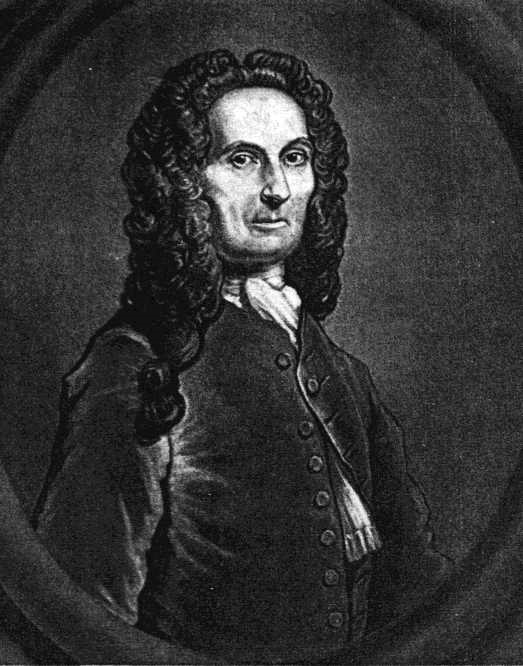
\includegraphics[scale=0.27]{figures/Abraham_de_moivre.jpeg}
%\legend{Fonte: Wikimedia Foundation, 2022.}
    \label{fig:my_label6} 
\end{figure}

%ABRAHAM DE MOIVRE. In: WIKIPÉDIA, a enciclopédia livre. Flórida: Wikimedia Foundation, 2022. Disponível em: <https://pt.wikipedia.org/w/index.php?title=Abraham_de_Moivre&oldid=64507244>. Acesso em: 4 out. 2022.

\vskip0.3cm 
Diversos autores consideram Laplace como tendo realizado as maiores contribuição à teoria da probabilidade, mas foi dado o nome de Gauss para a distribuição depois de ele tê-la aplicado a teoria dos movimentos dos corpos celestes.\vskip0.3cm 


Quando os valores das observações de uma variável resposta, originados de uma amostra, são agrupados em tabelas de frequências, objetiva-se conhecer a variação e como se processa a distribuição dos dados.\vskip0.3cm 



\newpage
Existem inúmeros tipos de curvas que podem representar as distribuições. Na maioria das pesquisas na Gestão Pública, as observações variam em torno da distribuição normal, a qual é uma distribuição contínua. É a mais importante distribuição no campo da Estatística e tem a seguinte função de densidade:\vskip0.3cm 


\begin{equation}
f\left(x\right) = \frac{1}{\sqrt{2\pi \sigma^2}}exp \left\{-\frac{1}{2}\left(\frac{x-\mu}{\sigma}\right)^2 \right\},~~~-\infty<x<\infty~~\text{e}~\sigma>0
 \end{equation} 

È uma curva estável, em forma de sino, e simétrica em torno da média da distribuição, simbolizada pela letra grega $\mu$ (mi). O desvio-padrão da distribuição é simbolizado pela letra grega $\sigma$ (sigma).\vskip0.3cm 


\begin{figure}
    \centering
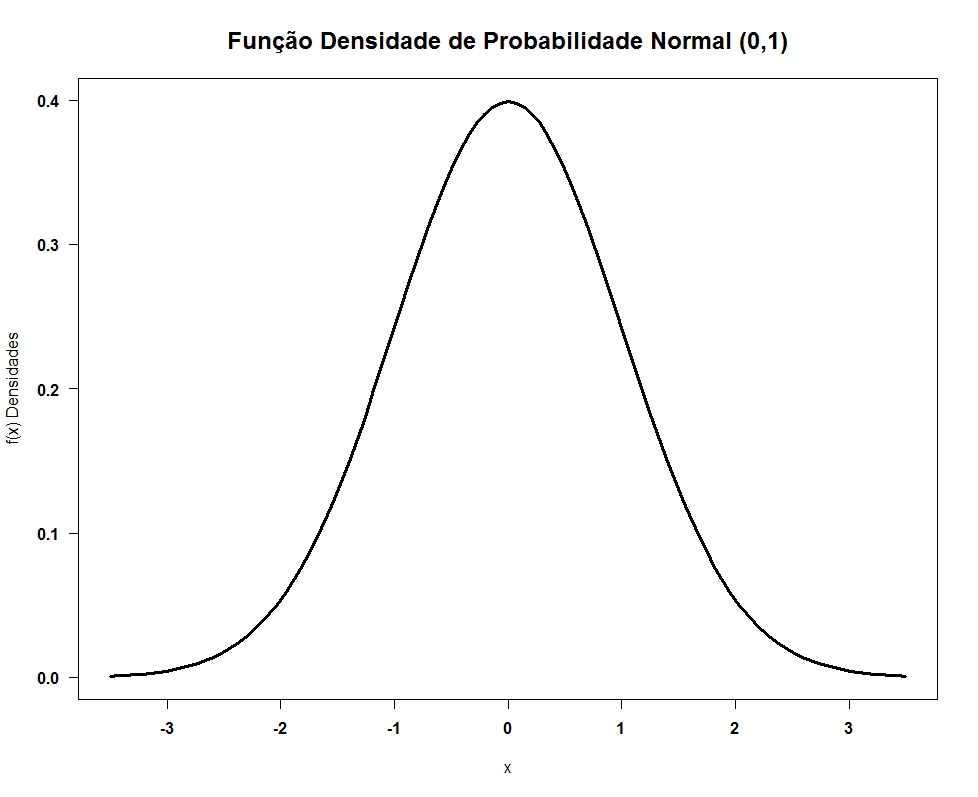
\includegraphics[scale=0.50,height=220pt,width=13cm]{figures/densidade1.jpeg}
    \caption{Função de Densidade de Probabilidade da Distrinuição Normal N(0,1).}
    \label{fig:my_label70}
\end{figure}


\newpage
\subsection{Distribuição $t$ de $Student$}
\subsubsection{A Origem da $t$ $student$}

William Sealy Gosset nasceu em 13 de junho de 1876 em Canterbury, Inglaterra, o primeiro de cinco filhos do Coronel Frederic Gosset e Agnes Sealy Vidal. Ele tinha problemas de visão e não conseguia seguir seu pai na Royal Engineers, mas ele era um aluno muito bom e ganhou várias bolsas de estudo.

\begin{figure}
    \centering
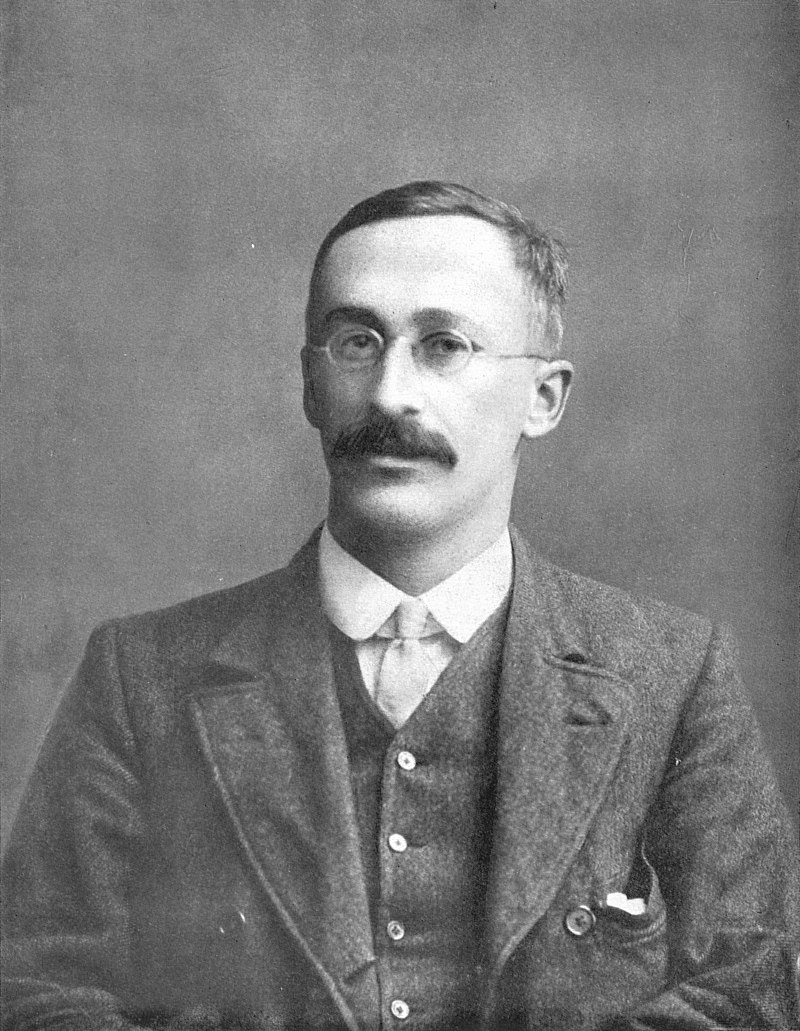
\includegraphics[scale=0.18]{figures/William_Sealy_Gosset.jpeg}
    \caption{William Sealy Gosset(1876-1937).}
    \label{fig:my_label3}
\end{figure}



Ao final do século XIX, a famosa \textbf{Arthur Guinness Son and Company} era a maior cervejaria do mundo, e foi pioneira em diversos esforços para o Controle de Qualidade. Em 1899, um dos contratados para o cargo de químico, recém-formado na Universidade de Oxford, com 23 anos de idade e um currículo que combinava matemática e estatística, foi \textbf{William Sealy Gosset}.\vskip0.3cm

%\begin{figure}[!htb]
%\centering{
% \includegraphics[scale=0.5]{figures/Gosset2.png}\\
%  \vspace{-0.8cm}
%  \caption{William Sealy Gosset, 1908}\label{esquematabela1}}
%\end{figure}


A \textit{Guinness} era uma empresa de Agro-Química progressista e Gosset iria aplicar os seus conhecimentos de estatística tanto na cervejaria (a destilaria) como nas quintas, para a selecção dos melhores espécimens de cevada.\vskip0.3cm

\newpage
O trabalho de Gosset na Guinness consistia em medir os inúmeros fatores do processo de produção e ponderar como eles se relacionam aos resultados do produto final. William realizou muitos testes para estimar a duração da cerveja diante das diferentes condições de armazenagem, fabricação e transporte.\vskip0.3cm


Gosset desenvolveu o teste t, distribuição passível de ser tabulada, como um modo barato de monitorar a qualidade da cerveja. Na época, não existia uma teoria para a tomada de decisões com base em pequenas amostras. Por isso, o grande diferencial desse teste é justamente permitir que se façam inferências usando um menor número de elementos. \vskip0.3cm

Um outro funcionário da Guinness tinha já publicado um trabalho que continha alguns segredos da Cervejeira Guinness. Para prevenir fugas de informação e futuras revelações dos "segredos" da marca, a Guinness proibiu que os seus empregados pudessem publicar quaisquer trabalhos independentemente do conteúdo. Isto queria dizer que Gosset não tinha como publicar os trabalhos com o seu nome. Então, usou o pseudonimo $Student$ para as suas publicações evitando ser detectado pela entidade empregadora. \vskip0.3cm

Desta forma, o seu feito mais conhecido, é hoje conhecido com a Distribuição t-Student, que noutras circunstâncias seria conhecida como a Distribuição t-Gosset.\vskip0.3cm


Gosset trabalhou na cervejaria em St. James's Gate por 36 anos, antes de se tornar o cervejeiro-chefe de uma nova cervejaria Guinness em Park Royal em Londres. Em outubro de 2012, uma placa foi inaugurada na Escola Nacional de St Patrick, Blackrock(Irlanda), para homenagear William Sealy Gosset, que morou nas proximidades por 22 anos. 


\begin{figure}
    \centering
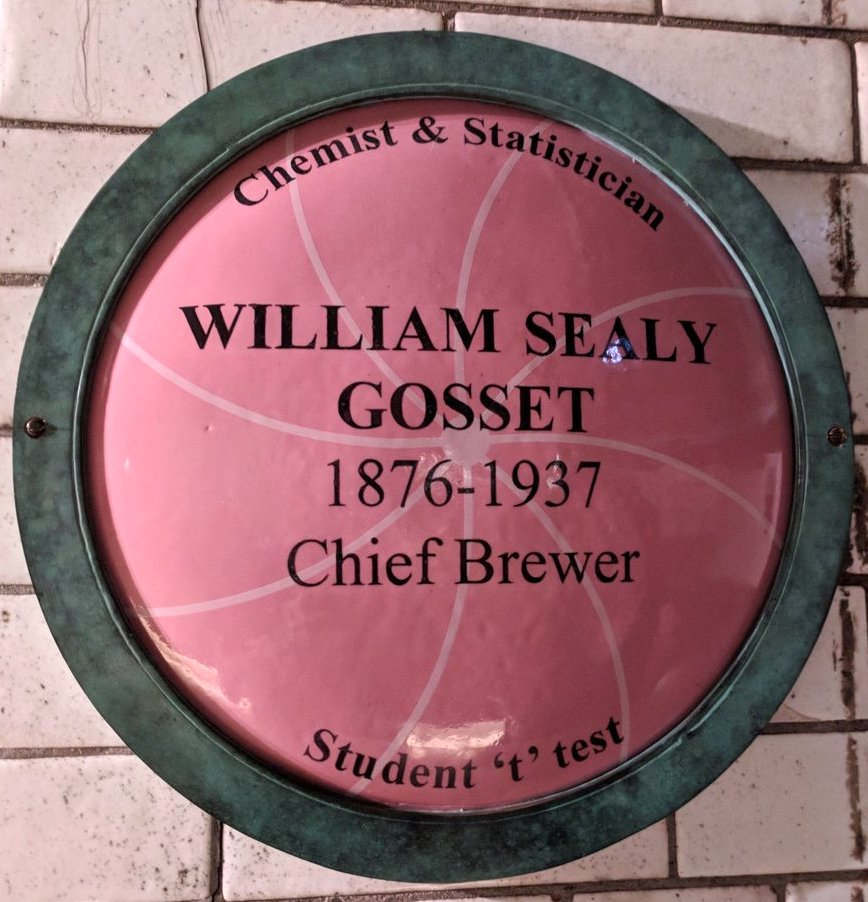
\includegraphics[scale=0.13]{figures/Gosset_plaque_in_Guinness.jpg}
    \caption{Placa no Guinness Storehouse em homenagem a Gosset.}
    \label{fig:my_label3}
\end{figure}



\newpage
\subsubsection{A Distribuição $t$ \textit{student}}

Seja a variável aleatória:

\begin{equation}
    t =\frac{\overline{y}-\overline{Y}}{\frac{s(Y)}{\sqrt(n)}}
\end{equation}

Esta variável é conhecida com distribuição $t$ student, com $k=n-1$ graus de liberdade, podendo também ser escrita na forma:

\begin{equation}
    t =\frac{N(0,1)}{\sqrt{\frac{\chi^{2}_{n-1}}{n-1}}}
\end{equation}

O $s(y)$ é considerado o desvio-padrão estimado.\vskip0.3cm

O gráfico da função densidade da variável $t$ de student é simétrico e tem uma forma parecida com a distribuição normal, entretando, menos achatada, com a média zero e variância igual $\frac{k}{(k-2)}$, em que $k>2$ graus de liberdade. A função densidade da variável $t$ é dada pela expressão (2.10). 

\begin{equation}
f\left(t\right)=\frac{1}{\sqrt{k \pi}}\frac{\Gamma\left(\frac{k+1}{2}\right) }{\Gamma \left(\frac{k}{2}\right)}\left(1+\frac{t^2}{k}\right)^{-\left(\frac{\upsilon+1}{2}\right)},~~~-\infty<x<\infty
\end{equation}

Sir \textbf{Ronald Fisher} o arquiteto da estatística experimental, um gigante entre os estatísticos, chamou Gosset de “O Faraday das Estatísticas”, reconhecendo sua capacidade de compreender princípios gerais e aplicá-los a problemas de importância prática (SALSBURG, 2000).


\newpage
\subsubsection{Ronald Aylmer Fisher}

Ronald Aylmer Fisher foi um estatístico, biológo e geneticista, nasceu em 17 de fevereiro de 1890, em East Finchley, Londres, sendo considerado um dos pais e o fundador da estatística moderna (BOX, 1978).\vskip0.3cm


Fisher bacharelou-se em mamtemática pela Universidade de Cambridge, e que no início do século XX, em 1919, chefiou um laboratório de Estatística Experimental de Agricultura, chamado centro de experimentos de Rothamsted Research em Harpenden na Inglaterra, onde permaneceu até 1933 (SALSBURG, 2000).

\vspace{-0.3cm}

\begin{figure}
    \centering
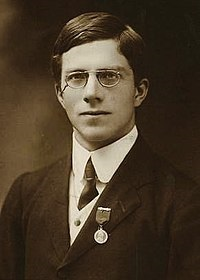
\includegraphics[scale=0.9]{figures/fisher.jpeg}
    \caption{Ronald Aylmer Fisher(1890-1962).}
    \label{fig:my_label3}
\end{figure}


Ronald Fisher nesse período se dedicou e estudou, diariamente, os problemas do planejamento e análise de pesquisa na àrea agrária. \vskip0.3cm


O grande fascínio de fisher pelos problemas de pesquisa, em ciências agrárias, trouxe a inspiração para desenvolver os métodos de análise de Delineamentos Experimentais, a \textbf{Análise de Variância}, que em conjunto com a \textbf{Análise de Covariância}, também de sua autoria, constitui-se no instrumento fundamental para a interpretação das análises dos resultados dos experimentos planejados (SALSBURG, 2000). \vskip0.3cm


% Hald, Anders (1998). A History of Mathematical Statistics. Nova York: Wiley
% SALSBURG, David. The Lady Tasting Tea: How Statistics Revolutionized Science in the Twentieth Century, 2000
% Dawkins, Richard (1995). River out of Eden. [S.l.: s.n.]
% BOX, Joan Fisher. R. A. Fisher: The Life of a Scientist. Nova York: Wiley, 1978.

\newpage
Foi descrito por Anders Hald como "um gênio que criou praticamente sozinho as fundações para a moderna ciência estatística (HALD, 1998) e Richard Dawkins, que o descreveu como "o maior dos sucessores de Darwin" (DAWKINS, 1995).\vskip0.3cm

Ronald Fisher recebeu vários prêmios importantes ao longo de sua carreira, tais como:

\begin{itemize}
    \item \textbf{Prêmio Memorial Weldon:} é concedido anualmente pela Universidade de Oxford para notáveis contribuições no desenvolvimento de métodos matemáticos ou estatísticos aplicados à problemas em biologia; 
    \item \textbf{Medalha Real (1938):} é entregue anualmente pelo Monarca do Reino Unido para contribuições dos avanços do conhecimento da Natureza;
    \item \textbf{Medalha Guy de Ouro (1946):} é concebida pela Royal Statistical Society em três categorias: ouro, parata e bronze; A medalha de ouro é concebida a contribuição inovativa à teoria estatística e suas aplicações;
    \item \textbf{Medalha Copley (1955):} É a medalha de maior prestígio atribuída pela Royal Society.
    \item \textbf{Medalha Darwin-Wallace (1958):} é uma medalha oferecida pela Linnean Society of London a cada 50 anos, por grande contribuições nos avanços para biologia evolucionista.
\end{itemize}




